\documentclass[12pt,letterpaper]{article}

\usepackage{ifpdf}
\usepackage[utf8]{inputenc}
\usepackage{times}
\usepackage{graphicx}
\usepackage{setspace}
\usepackage{float}

\usepackage{anysize}
\marginsize{1in}{1in}{1in}{1in}

% Resize section titles
\usepackage{titlesec}
\titleformat{\section}{\large\bfseries}{\thesection}{1em}{}
\titleformat{\subsection}{\bfseries}{\thesection}{1em}{}

% "<author> <page>" style page headers
\usepackage{fancyhdr}
\fancypagestyle{norule}{ %
    \renewcommand{\headrulewidth}{0pt}
    \renewcommand{\footrulewidth}{0pt}
}
\fancyhf{}
\pagestyle{norule}
\rhead{Cesare \thepage}
\setlength\headsep{0.333in}

% Works cited environment
% (to start, use \begin{workscited...}, each entry preceded by \bibent)
%  - from Ryan Alcock's MLA style file
\newcommand{\bibent}{\noindent \hangindent 40pt}
\newenvironment{workscited}{\newpage\begin{center} \large\bfseries Works Cited \end{center} \doublespacing}{\newpage}

\DeclareGraphicsExtensions{.png}

\begin{document}

% Header
\begin{flushleft}
  Kyle Cesare \\
  WR327, Section 016\\
  February 18, 2013
\end{flushleft}

% No header on the first page
\thispagestyle{empty}

\begin{center}
  \Large \textbf{Building Software with the Waterfall Design Pattern}
\end{center}

% Describe/define the process to be analyzed. State the purpose and scope of the
% document. Present a statement of organization that describes the contents of
% this paper.
\section*{Introduction}
The waterfall software development model is a process for developing software
often used when it is important the software be correct on the initial
development pass (Fairley 55).  The purpose of this document is to help the
reader to understand the process so he or she may use it more effectively.  This
document will only outline the process from a technology-agnostic point of view.
It will not delve into how each step is to be executed based on a specific
software platform.  I will first cover some background information on the
waterfall model.  Then, I will go in-depth about each step of the process.
Finally, I will summarize the material covered.

% Provide contextual information required for your reader to understand the
% process. For example,if you’re describing the process for creating steel
% girders, you might explain how girders are used or you might explain how the
% creation process fits into the larger process of using them in construction.
% Conclude this section with a sentence or two which breaks the process into
% stages: "The principle stages of creating an I-beam are smelting, casting,
% forming, and prepping for shipment."
\section*{Background}
The waterfall model was first conceived in 1970 by Winston Royce in his seminal
paper ``Managing the Development of Large Software Systems: Concepts and
Techniques'' (Fairley 55).  While other software development processes, like the
agile model, focus on multiple cycles and iterations of development, the
waterfall model's goal is to complete the system in one pass of a linear
sequence, as is shown in figure~\ref{waterfall} (Hanna).  Note that different
authors may label steps differently, but the process usually remains unchanged.

\begin{figure}[H]
  \centering
  \caption{Waterfall Design Model Outline.  Steven Zeil \copyright 1998-2008.\label{waterfall}}
  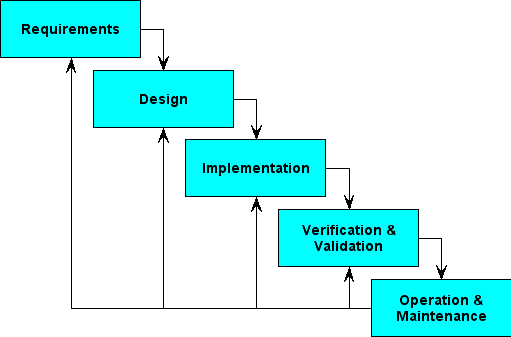
\includegraphics[width=4in]{waterfall}
\end{figure}

Regardless of terminology, the process can be broken down into six steps.
First, the developers must meet with the client and determine what will be
developed.  Then, the developers must design the software.  Third, individual
modules are developed, and then pulled together in the fourth step.  The product
must then be tested.  Finally, for the remainder of the product's life cycle, it
must be maintained.

% Step-by-step description. Each step should include a definition of the step,
% the purpose or function within the process, any necessary contextual
% information, and any necessary brief mechanical description for any components
% invovled.
\section*{Process Description}
The waterfall software development model is broken into six steps that must be
followed sequentially.

\subsection*{1. Requirements specification}
The development team meets with the client to create a document detailing all
features, expected behaviors, and metrics of the software.  This is necessary
because the development team does not meet with the client until the final
product is verified.  Any mistakes in the requirement specification will likely
not be found until much later, and may have considerable consequences.  A
requirements document for a website should discuss thoroughly how the website is
supposed to look, what every page is supposed to do, and any performance or
resource usage metrics that must be met.

\subsection*{2. Design}
The development team, perhaps in collaboration with a software architect, build
design documents that may include data flow charts, user experience storyboards,
and platform technology analyses.  Developers may use standardized methods like
the Unified Modeling Language to more easily communicate with other teams.
Without the design step, it would be very difficult to start implementing the
software as the developers would have no idea of the system's layout and
interfaces.  If a website was being developed, the developers would need to
conduct usability studies, model the storage and flow of data throughout the
program, and decide on a technology stack for implementation.

\subsection*{3. Construction}
The developers take what they have learned from the design stage and write the
code.  This is the most important step of the entire process, and is what every
other step either builds up to or works off of.  Depending on the development
team and type of software being built, a team might write code in C using the
Windows API and share code using a distributed version control system, like
Mercurial or Team Foundation Server.

\subsection*{4. Integration}
The developers now combine the individual modules developed in the construction
phase to build the final piece of software.  Without this step, the entire
system would have to be built in one piece.  This is very prone to error and is
extremely risky if the design is found to be faulty.  In the website example,
the team might need to integrate the database layer written in SQL with the
logic layer, in C, and then connect that to the presentation layer designed in
HTML.

\subsection*{5. Testing}
The development team must now ensure that their system works as desired, and
that it meets the client's requirements.  This is accomplished by writing test
suites and performing acceptance testing with the client.  It is important to
ensure the client likes the final product because developers often lose sight of
the average user and build the software based on the use case of a developer.
For the website development example, the development team could use browser
automation testing tools to verify functionality.  They would then meet with the
client and demonstrate that they have fully implemented the system as outlined
by the requirements document.

\subsection*{6. Maintenance}
In the longest step of the entire process, developers must continue to provide
support for the software, even long after it has been shipped.  This step is
extremely important, as some bugs and flaws do not show themselves until the
software is deployed in production.  A website development team may find that
their database layer is not reaching the required performance once the database
has been populated with millions of records, so they must rethink portions of
their design and publish an update.

% Recap the major steps in the process and describe the outcome, product, or
% effect of the overall process.
\section*{Conclusion}
As has been shown, the waterfall software development process is comprised of
six steps.  First, the developers meet with the client and draft the
requirements.  Then, the developers design the software, construct it, and
integrate it into a functioning product.  They must then test it.  Finally, they
must maintain it for the rest of its life cycle.  By following this process,
teams can more efficiently, both in terms of time and money, develop large
software products.

\begin{workscited}

\bibent Fairley, Richard E. Managing and Leading Software Projects. Chicester:
Wiley, 2009. Print.

\bibent Hanna, Mary. ``Farewell to waterfalls?'' Software Magazine May 1995:
38+.  Academic OneFile. Web. 14 Feb. 2013.

\bibent Zeil, Steven J. ``Software Development: The Waterfall Model.'' Old
Dominion University, 2008. Web. 14 Feb. 2013.

\end{workscited}
\end{document}
